\documentclass[a4paper, 10pt, twoside]{article}

\usepackage[top=1in, bottom=1in, left=1in, right=1in]{geometry}
\usepackage[utf8]{inputenc}
\usepackage[spanish, es-ucroman, es-noquoting]{babel}
\usepackage{setspace}
\usepackage{fancyhdr}
\usepackage{lastpage}
\usepackage{amsmath}
\usepackage{amsfonts}
\usepackage{amsthm}
\usepackage{verbatim}
\usepackage{fancyvrb}
\usepackage{graphicx}
\usepackage{float}
\usepackage{enumitem} % Provee macro \setlist
\usepackage{tabularx}
\usepackage{multirow}
\usepackage{hyperref}
\usepackage{xspace}
\usepackage{graphicx}
\usepackage[rightcaption]{sidecap}
\usepackage{ulem} % Provee macro \uwave
\usepackage[toc, page]{appendix}
\usepackage{titlesec}
\usepackage{relsize}
\setcounter{secnumdepth}{4}

\usepackage{tikz}
\usetikzlibrary{decorations.markings,arrows}


%%%%%%%%%% Constantes - Inicio %%%%%%%%%%
\newcommand{\titulo}{Trabajo Práctico 3}
\newcommand{\materia}{Métodos Numéricos}
\newcommand{\integrantes}{Martinez · Fixman · Baca  Paunero}
\newcommand{\cuatrimestre}{Segundo Cuatrimestre de 2015}
%%%%%%%%%% Constantes - Fin %%%%%%%%%%

\titleformat{\paragraph}
{\normalfont\normalsize\bfseries}{\theparagraph}{1em}{}
\titlespacing*{\paragraph}
{0pt}{3.25ex plus 1ex minus .2ex}{1.5ex plus .2ex}

%%%%%%%%%% Configuración de Fancyhdr - Inicio %%%%%%%%%%
\pagestyle{fancy}
\thispagestyle{fancy}
\lhead{\titulo}
\rhead{\integrantes}
\renewcommand{\footrulewidth}{0.4pt}
\cfoot{\thepage /\pageref{LastPage}}

\fancypagestyle{caratula} {
   \fancyhf{}
   \cfoot{\thepage /\pageref{LastPage}}
   \renewcommand{\headrulewidth}{0pt}
   \renewcommand{\footrulewidth}{0pt}
}
%%%%%%%%%% Configuración de Fancyhdr - Fin %%%%%%%%%%


%%%%%%%%%% Miscelánea - Inicio %%%%%%%%%%
% Evita que el documento se estire verticalmente para ocupar el espacio vacío
% en cada página.
\raggedbottom

% Separación entre párrafos.
\setlength{\parskip}{0.5em}

% Separación entre elementos de listas.
\setlist{itemsep=0.5em}

% Asigna la traducción de la palabra 'Appendices'.
\renewcommand{\appendixtocname}{Apéndices}
\renewcommand{\appendixpagename}{Apéndices}
%%%%%%%%%% Miscelánea - Fin %%%%%%%%%%



\begin{document}


%%%%%%%%%%%%%%%%%%%%%%%%%%%%%%%%%%%%%%%%%%%%%%%%%%%%%%%%%%%%%%%%%%%%%%%%%%%%%%%
%% Carátula                                                                  %%
%%%%%%%%%%%%%%%%%%%%%%%%%%%%%%%%%%%%%%%%%%%%%%%%%%%%%%%%%%%%%%%%%%%%%%%%%%%%%%%


\thispagestyle{caratula}

\begin{center}


\includegraphics[height=2cm]{DC.png}
\hfill

\includegraphics[height=2cm]{UBA.jpg}

\vspace{2cm}

Departamento de Computación,\\
Facultad de Ciencias Exactas y Naturales,\\
Universidad de Buenos Aires

\vspace{4cm}

\begin{Huge}
\titulo
\end{Huge}

\vspace{0.5cm}

\begin{Large}
\materia
\end{Large}

\vspace{1cm}

\cuatrimestre

\vspace{4cm}

\begin{tabular}{|c|c|c|}
\hline
Apellido y Nombre & LU & E-mail\\
\hline
Martinez, Federico.  & 191/10 &  fedomartinez@hotmail.com\\
Fixman, Martin      & 391/11 & martinfixman@gmail.com\\
Baca Paunero, Juan & 690/06 & wencesj@gmail.com\\
\hline
\end{tabular}

\end{center}

\newpage

\tableofcontents

\newpage

\section{Introducción}

En esta secci\'on realizaremos una breve descripci\'on te\'orica acerca de los temas a tratar en este trabajo, con la finalidad de tener una idea clara de los mismos para poder tener un mejor entendimiento de lo realizado.

\subsection{¿Qu\'e es un video digital?}

Un video est\'a compuesto por cuadros (denominados tambi\'en frames en ingl\'es) donde cada uno de ellos es una imagen. El ojo humano es capaz de distinguir aproximadamente 20 im\'agenes por segundo. De este modo, cuando se muestran m\'as de 20 imágenes por segundo, es posible enga\~nar al ojo y crear la ilusi\'on de una imagen en movimiento. La fluidez de un video se caracteriza por el número de im\'agenes por segundo (frecuencia de cuadros), expresado en \textbf{FPS} (cuadros por segundo). 

\subsection{Videos en c\'amara lenta}

La c\'amara lenta es un efecto visual que permite retrasar artificialmente una acci\'on con el fin de aumentar el impacto visual o emocional. La c\'amara lenta se obtiene rodando una escena con un n\'umero de im\'agenes por segundo superior a la velocidad de proyecci\'on. Al pasar el registro con un n\'umero de im\'agenes por segundo normal, la escena, m\'as larga, da la impresión de desarrollarse lentamente. Por lo general las tomas de c\'amara lenta se generan con c\'amaras que permiten tomar alt\'isimos nu\'meros de cuadros por segundo, unos 100 o m\'as en comparaci\'on con entre 24 y 30 que se utilizan normalmente.

Nuestro trabajo se centrar\'a en este tipo de videos. Utilizando diferentes t\'ecnicas, crearemos cuadros artificiales a partir de los originales para generar el efecto de la c\'amara a partir de videos que no son de c\'amara lenta. Utilizaremos im\'agenes  en escala de grises para disminuir los costos en tiempo necesarios para procesar los datos y simplificar la implementaci\'on; sin embargo, la misma idea puede ser utilizada para videos en color.

\subsection{M\'etodos de generaci\'on de cuadros}

Para la generaci\'on de cuadros extra construiremos, para cada posici\'on (i,j), los valores de los cuadros agregados en funci\'on de los cuadros conocidos. Lo que haremos ser\'a interpolar en el tiempo y para ello consideraremos los siguientes tres m\'etodos de interpolaci\'on:

\begin{enumerate}
\item \textbf{Vecino m\'as cercano:} Consiste en rellenar el nuevo cuadro replicando los valores de los p\'ixeles del cuadro original que se encuentra m\'as cerca.
\item \textbf{Interpolaci\'on lineal:} Consiste en rellenar los p\'ixeles utilizando interpolaciones lineales entre p\'ixeles de cuadros originales consecutivos.
\item \textbf{Interpolaci\'on por Splines:} Similar al anterior, pero considerando interpolar utilizando splines y tomando una cantidad de cuadros mayor.
\end{enumerate}

Durante el desarrollo del trabajo, analizaremos las caracter\'isticas, ventajas y desventajas particulares de cada uno de los m\'etodos. 

\subsection{Conceptos relevantes para el desarrollo}

Para realizar un an\'alisis cuantitativo, llamaremos F al frame del video real (ideal) que deber\'iamos obtener con nuestro algoritmo, y $\overline{F}$ al frame del video efectivamente construido. Consideramos entonces dos medidas, directamente relacionadas entre ellas, como el \textbf{Error Cuadr\'atico Medio} (ECM) y \textbf{Peak to Signal Noise Ratio} (PSNR), denotados por ECM(F, $\overline{F}$) y PSNR(F, $\overline{F}$), respectivamente, y definidos como:

$ECM(F, \overline{F}) = \frac{1}{mn} \sum\limits_{i=1}^m\sum\limits_{j=1}^n |F_{k_{ij}} - \overline{F}_{k_{ij}}|^2$ (1)

y

$PSNR(F, \overline{F}) = 10log_{10}(\frac{255^2}{ECM(F,\overline{F})})$

Donde $m$ es la cantidad de filas de p\'ixeles en cada imagen y $n$ es la cantidad de columnas.

\section{Desarrollo}

\section{Desarrollo}

\subsection{Consideraciones Generales}

Cada video est\'a compuesto por frames de $h$ pixeles de altura y $w$ pixeles de
ancho, donde cada pixel es un valor entero del $0$ al $255$, inclusive. A la
vez, se consideran $c0$ de estos frames en suceci\'on para formar el video.

Para alentar el video nosotros tomamos un factor $q > 1$ (equivalente al
argumento $c + 1$), y generamos un video con $c1 = (c0 - 1) * q + 1$ frames. A cada frame
le aplicamos cierto \textit{m\'etodo}, dependiendo de nuestras restricciones,
para aproximar los frames restantes entre el video original y el video alentado.

Cada uno de los m\'etodos que usamos opera con un solo pixel y el cambio de su
valor a trav\'es del tiempo, as\'i que no es necesario que conozca todo un frame
entero. Por esto, definimos cada m\'etodo como una funci\'on que toma dos
par\'ametro:

\[
\begin{split}
P \in \mathbb{P}^{c_0} & : \text{un vector de pixeles (valores en $[0, 255]$)} \\
c1 \in \mathbb{N} & : \text{la cantidad de frames en la pel\'icula resultante}
\end{split}
\]

Y a la vez devuelve un par\'ametro del tipo

\[
A \in \mathbb{P}^{c_1} : \text{el pixel $P$ en la pel\'icula final}
\]

El enunciado tambi\'en especifica el par\'emtro $f$, el framerate del video,
pero adem\'as de hacerle una transformaci\'on simple al video final no influye a
ninguno de nuestros m\'etodos.

Durante el resto de la resoluci\'on usamos t\'erminos como ``cercano'' y
``lejano''. Se debe entender que, como los m\'etodos trabajan sobre un solo
pixel y como cambia en el tiempo, estos se refieren a t\'erminos t\'emporales y
no espaciales.

\subsection{Vecino M\'as Cercano}

El m\'etodo del vecino m\'as cercano implica, por cada pixel en la imagen
resultante, darle el valor del pixel m\'as cercano \footnote{temporalmente} en
la imagen original. Para lograr esto, podemos definirlo como la siguiente
sucesi\'on:

\[
A_i = P_{\left[i / \frac{c_1 - 1}{c_0 - 1}\right]}
\]

Donde $\left[x\right]$ representa el redondeo de $x$ al entero m\'as cercano.

\subsection{Interpolaci\'on Lineal}

El m\'etodo de la interpolaci\'on lineal consiste en crear una funci\'on lineal
entre cada par de pixeles consecutivos \footnote{de nuevo, en el sentido
temporal} de $P$, y estimar los valores del vector $A$ desde el valor que toma
cada funci\'on en los puntos intermedios.

La funci\'on lineal entre dos puntos $\left(x_0, y_0\right)$ y $\left(x_1,
y_1\right)$ debe satisfacer la f\'ormula

\[
\frac{y - y_0}{x - x_0} = \frac{y_1 - y_0}{x_1 - x_0}
\]

Por lo tanto, podemos definir la funci\'on $f$ que represente la interpolaci\'on
lineal entre esos dos puntos como

\[
f(x) = y_0 + (y_1 - y_0) \frac{x - x_0}{x_1 - x_0}
\]

Como debemos definir esta f\'ormula las interpolaciones entre varios puntos en
el plano discreto, definimos el m\'etodo como la sucesi\'on

\[
q = (c1 - 1) / (c0 - 1)
\]

\[
\forall{i < c_1}
\begin{split}
& x_0_i = \floorl \frac{i}{q} \floorr \\
& y_0_i = P_{x_0_i} \\
& x_1_i = \ceill \frac{i}{q} \ceill \\
& y_1_i = P_{x_1_i} \\
& A_i = y_0_i + (y_0_i - y_1_i) * \frac{i - x_0_i}{x_1_i - x_0_i}
\end{split}
\]

\subsection{Interpolaci\'on por Splines}

En este m\'etodo definimos un spline c\'ubico n\'atural $S$ que interpole todos
los valores en $P$ para lograr conseguir los valores intermedios de $A$.
Nosotros definimos este spline como una funci\'on ``flu\'ida'' que pase por
todos los puntos $(x_0, y_0)$ definidos en $P$. Para lograr esto, separamos $S$
en diferentes subfunciones, $S_{0 \ldots c_0 - 1}$ tal que cada partici\'on sea
un polinomio c\'ubico definido entre dos puntos de $P$, y la derivada primera y
segunda de cada par consecutivos sean iguales. En otras palabras,

\[
\begin{split}
S(x) & =
\begin{cases}
	S_0(x) & \text{si } x \in [x_0, x_1] \\
	\vdots \\
	S_{c_1 - 1} \text{si } x \in [x_{n - 1}, x_n]
\end{cases} \\
S_i(x) & = a_i + b_i(x - x_i) + c_i(x - x_i)^2 + d_i(x - x_i)^3 \\
S_i(x_i + 1) & = S_{x + 1}(x_i + 1) \forall i \in [0, n - 2] \\
S'_i(x_i + 1) & = S'_{x + 1}(x_i + 1) \forall i \in [0, n - 2] \\
S''_i(x_i + 1) & = S''_{x + 1}(x_i + 1) \forall i \in [0, n - 2] \\
S''(x_0) & = S''(x_n) = 0
\end{split}
\]

Como en cada $x_i$ $S(x_i) = S_i(x_i)$ y $S_i(x_i) = a_i$, podemos ver que

\[
a_i = y_i
\]

Tambi\'en, ya que $S_i(x_i + 1) = y_{i + 1}$,

\[
a_i + b_i(x_{i + 1} - x_i) + c_i(x_{i + 1} - x_i)^2 + d_i(x_{i + 1} - x_i)^3 = a_{i + 1}
\]

Derivando cualquier polinomio c\'ubico $S_i$ obtenemos que

\[
\begin{split}
S_i'(x) & = b_i + 2 c_i (x - x_i) + 3 d_i (x_(i + 1) - x_i)^2 \\
S_i''(x) & = 2 c_i + 6 d_i (x - x_i)
\end{split}
\]

Por lo tanto, ya que las derivadas primera y segunda de los polinomios
consecutivos deben ser iguales,

\[
b_i + 2 c_i (x_{i + 1} - x_i) + 3 d_i (x_{i + 1} - x_i)^2 = b_{i + 1}
\]

\[
2 c_i + 6 d_i (x_{i + 1} - x_i) = 2 c_{i + 1}
\]

Y, como el spline es n\'atural y la derivada segunda en el primer y \'ultimo
punto debe ser $0$,

\[
2 c_0 = 0
\]

\[
2 c_{n - 1} + 6 d_{n - 1} (x_n - x_{n - 1}) = 0
\]

Resumiendo, y sabiendo que $x_{i + 1} - x_i = q \forall i \in [0, n - 2]$
tenemos las siguientes ecuaciones i para los factores de los polinomios:

\begin{enumerate}
\item $ a_i = y_i $
\item $ a_i + b_i q + c_i q^2 + d_i q^3 $
\item $ b_i + 2 c_i q + 3 d_i h_i^2 = b_{i + 1} $
\item $ 2 c_i + 6 d_i q = 2 c_{i + 1} $
\item $ c_0 = 0 $
\end{enumerate}

Despejando la ecuaci\'on 4, obtenemos

\[
d_i = \frac{1}{3 q} c_{i + 1} - c_i
\]

Y sustituyendo este $d$ y el $a$ de la ecuaci\'on 1 en la ecuaci\'on 2 obtenemos
que

\[
\begin{split}
b_i & = \frac{1}{q} (y_{i + 1} - y_i - c_i q^2 - d_i q^3) \\
& = \frac{1}{q} (y_{i + 1} - y_i - c_i q^2 - \frac{1}{q} (c_{i + 1} - c_i) q^3 \\
& = \frac{1}{q} (y_{i + 1} - y_i) - c_i q \frac{1}{3} (c_{i + 1} - c_i) q \\
& = \frac{1}{q} * (y_{i + 1} - y_i) - \frac{q}{3} (2 c_i + c_{i + 1})
\end{split}
\]

Substituyendo el valor de $b_i$ en la ecuaci\'on 3,

\[
\begin{split}
0 & = b_i - b_{i + 1} + 2 c_i q + 3 d_i q^2 \\
& = \frac{1}{q} (y_{i + 1} - y_i) - \frac{q}{3} (2 c_i + c_{i + 1}) - \frac{1}{q} (y_{i + 2) - y_{i + 1}} + \frac{q}{3} (2 c_{i + 1} + c{i + 2}) + 2 c_i q + q (c_{i + 1} - c_i)
& = \left[ \frac{1}{q} (y_{i + 1} - y_i) - \frac{1}{q} (y_{i + 2} - y_{i + 1}) \right] + \frac{2}{3} q c_i - \frac{1}{3} q c_{i + 1} + \frac{2}{3} q c_{i + 1} + \frac{1}{3} q c_{i + 2} + 2 q c_i + q c_{i + 1} - q c_i
& \frac{1}{q} \left[ y_{i + 2} - 2 y_{i + 1} + y_i \right] + \frac{1}{3} q c_i + \frac{4}{3} c_{i + 1} + \frac{1}{3} q c_{i + 2}
\end{split}
\]

Equivalentemente,

\[
q c_i + 4 q c_{i + 1} + q c_{i + 2} = \frac{3}{q} \left[ y_{i + 2} - 2 y_{i + 1} + y_i \right]
\]

Esto es un sistema de $n - 1$ ecuaciones con $n + 1$ incognitas ($c_0 \cdots
c_n$). Tomando $c_0 = 0$ y $c_n = 0$ tenemos un sistema de $n + 1$ ecuaciones
que se puede expresar matricialmente de la forma

\[
Q * c = v
\]

Con

\[
Q \in \mathbb{R}^{(n + 1) \times (x + 1)}
\]
\[
Q = \begin{bmatrix}
1 & 0 & 0 & 0 \\
q & 4 q & 4 q & 0 \\
0 & q & 4 q & q \\
&&&& \xddots \\
&&&&& q & 4 q & q \\
&&&&& 0 & 0 & 1
\end{bmatrix}
\]

\[
c \in \mathbb{R}^{n + 1}
\]
\[
c = \begin{bmatrix}
c_0 \\
c_1 \\
c_2 \\
\vdots \\
c_{n - 1} \\
c_n
\end{bmatrix}
\]

\[
f \in \mathbb{R}^{n + 1}
\]

\[
f = \frac{3}{q} \cdot \begin{bmatrix}
0 \\
y_0 - 2 y_1 + y_2 \\
y_1 - 2 y_2 + y_3 \\
\vdots
y_{n - 2} - 2 y{n - 1} + y_n \\
0
\end{bmatrix}
\]

$A$ es una matriz banda de ancho 1, ya que todos sus valores fuera de la
diagonal principal y las dos diagonales son iguales a $0$, y como es
estrictamente diagonal dominante es inversible; entonces hay una soluci\'on
\'unica al sistema.

M\'as a\'un, como $A$ es tridiagonal se puede guardar en una matriz esparsa que
contenga solo las diagonales y su complejidad espacial sea $\mathbb(O)(n)$ de
espacio. Tambi\'en, el sistema puede ser resuelto haciendo eliminaci\'on
Gaussiana sobre la matriz en complejidad temporal $\mathbb(O)(n)$.

Finalmente, haciendo resuelto este sistema de ecuaciones y consiguiendo los
$c_i$ de cada polinomio dentro del spline, podemos volver a las ecuaciones
anteriores y definir los otros parametros como

\[
\begin{split}
a_i & = y_i \\
b_i & = \frac{1}{q} (y_{i + 1} - y_i) - \frac{q}{3} (2 c_i + c_{i + 1})
d_i = \frac{1}{3 q} (c_{i + 1} - c_i)
\end{split}
\]

Para ayudar al an\'alisis, usamos un parametro extra para este m\'etodo,
$reset$ \'o $r$, que indica que los splines se definen entre $r$ puntos. Eso es,
$S_0 \ldots S_{r - 1}$ forman un spline, $S_r \ldots S_{2r - 1}$ forman otro,
etc. Por simplicidad, en el caso que el \'ultimo spline contenta menos de $r$
puntos lo unimos con el anterior.


\section{Experimentaci\'on}

En esta secci\'on evaluaremos los 3 m\'etodos implementados de manera de poder comparar su velocidad de corrida (complejidad), determinar la calidad de regeneraci\'on de videos, artifacts producidos, etc. . Para eso, no solo usaremos los videos provistos por la c\'atedra, sino que adem\'as hemos incluido otros 4 videos que, si bien no todos aparecer\'an en los gr\'aficos de resultados, nos servir\'an para sacar conclusiones sobre los comportamientos de los m\'etodos a partir de las caracter\'isticas del video. Estos 4 videos son los siguientes:

\begin{itemize}
\item \textbf{slowmovesscene.mp4}: Es una escena del conocido video BigBuckBunny que tiene la caracter\'itica de ser un video de movimientos lentos y suaves, con casi ning\'un cambio de c\'amara. Esto lleva a que la variaci\'on entre frames sea ligera. 
\item \textbf{fastmovesscene.mp4}: Este video es una escena de una pelea con movimientos de alta velocidad, lo cual significa que las diferencias entre frame y frame son notorias.
\item \textbf{nocamerachanges.mp4}: Este video no posee ning\'un cambio de c\'amara, y los movimientos dentro del mismo son moderados, lo cual impide que existan altos contrastes entre frames.
\item \textbf{camerachanges.mp4}: Es un video que posee grandes cantidades de cambios de c\'amara que originan fuertes contrastes entre frames continuos.
\end{itemize}

El porque de la selecci\'on de estos videos es la siguiente: dado que todos los m\'etodos generan frames entre cada par de frames del video de entrada, buscamos analizar como reaccionan los mismos cuando el par de frames que utilizan para generar los nuevos frames son, o muy parecidos entre s\'i (escenas lentas o de movimientos suaves), o notoriamento diferentes (cambios de c\'amara bruscos o escenas de alta velocidad). Adem\'as, creemos que los videos con cambios de c\'amara o de alta velocidad son m\'as propensos a producir los llamados ``artifacts'' cuando se alentan en gran medidad. 

A continuaci\'on, analizaremos como los 3 m\'etodos implementados var\'ian en tiempo y el error (\textbf{ECM} y \textbf{PSNR}) generado entre frames reconstruidos con estos m\'etodos contra los frames del video original.

\subsection {An\'alisis de ECM y PSNR}

En el trabajo medimos la calidad de los m\'etodos para hacer una c\'amara lenta
de los videos bajando algunos videos con diferentes propiedades de internet
(osea que tienen relevancia en el mundo real), y sacando todos los frames
excepto uno de cada $c$. Luego se aplica alguno de los m\'etodos para generar un
video nuevo, con la misma cantidad de frames que el video original, que
idealmente ser\'ia igual (aunque es matem\'aticamente imposible \footnote{por el
principio del palomar} que haya un m\'etodo perfecto para todos los videos).

Luego, para medir el error entre el nuevo video en c\'amara lenta y el video
original se usa uno de dos m\'etodos: el \textbf{Error Cuadr\'atico Medio} o ECM
y el \textbf{Peak Signal to Nouse Ratio} o PSNR, que se definen como

\[
ECM(F, \bar{F}) = \frac{1}{m n} \sum^m_{i = i} \sum^n_{j = 1} \left| F_{k_{i j}} - \bar{F}_{k_{i j}} \right|^2
\]
\[
PSNR(F, \bar{F}) = 10 \; log_{10} \left( \frac{255^2}{ECM(F, \bar{F}} \right)
\]

Con $n$ igual a la altura de la im\'agen y $m$ igual a su largo. Estos dos
valores son importantes ya que, aunque los m\'etodos trabajen
``individualmente'' en un solo pixel, y el resultado de estos ser\'ian lo mismo
corriendose en mismo video que individualmente, ya que las pruebas son con videos
reales.

Hicimos los an\'alisis sobre 3 de los videos que contenian propiedades
interesantes: \textit{camerachanges.mp4}, \textit{slowmovescene.mp4}, y
\textit{funnybaby.avi}, y sobre los tres algoritmos. Como los videos son
relativamente peque\~nos y, por ende, el m\'etodo de splines es r\'apido,
dejamos el parametro $r$ del m\'etodo, que controla cada cuantos frames se
vuelven a empezar los splines, igual a $\infty$, osea que se hace un solo spline
para cada pixel del video.

Para ver como se comportaban los algoritmos mediante en salto, medimos el
\textbf{ECM} de cada frame en videos con saltos de 1, 3, 5, 7, y 10 frames, y
calculamos su promedio dependiendo del video y del m\'etodo:

\begin{figure}[H]
\centering
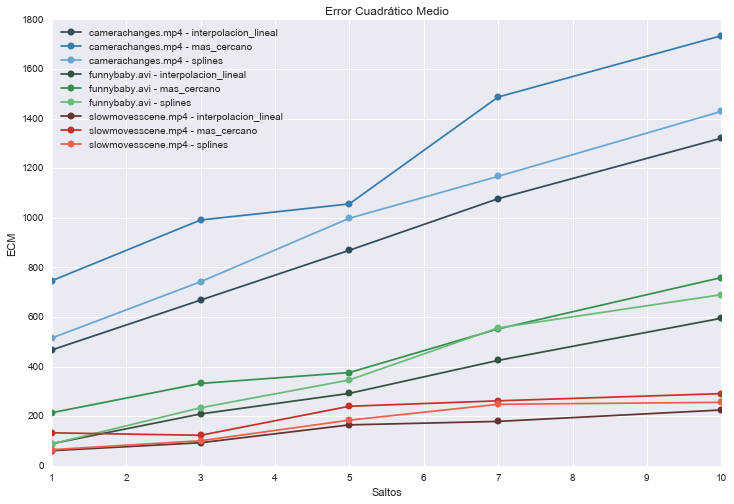
\includegraphics[width=.95\textwidth]{graficos/ecm.png}
\end{figure}

\vspace{-2em}
\begin{tiny}Este gr\'afico puede ser dificil de interpretar en blanco y negro\end{tiny}
\vspace{2em}

Este gr\'afico cementa la hipotesis de que \textit{camerachanges.avi}, que tiene
muchos cambios de c\'amara lo que hace que sea dificil predecir el valor de dos
pixeles cuando se pone en le c\'amara lenta tiene obviamente el mayor error. Por
otro lado, \textit{funnybaby.avi} y \textit{slowmoviescene.mp4} empiezan con un
\textbf{ECM} similar ya que ninguno de los dos tiene cambios bruscos, pero
cuando la cantidad de saltos aumenta el primer video empieza a tener un error
mucho mayor, ya que los cambios en el video dependientes del movimiento de la
cabeza del beb\'e \footnote{este es un beb\'e especialmente cabez\'on en comparaci\'on al
tama\~no del video} son mucho m\'as bruscos que los del video anterior.

Para comparar los m\'etodos, podemos ver el gr\'afico anterior y uno que tenga
solamente los valores para \textit{funnybaby.avi}

\begin{figure}[H]
\centering
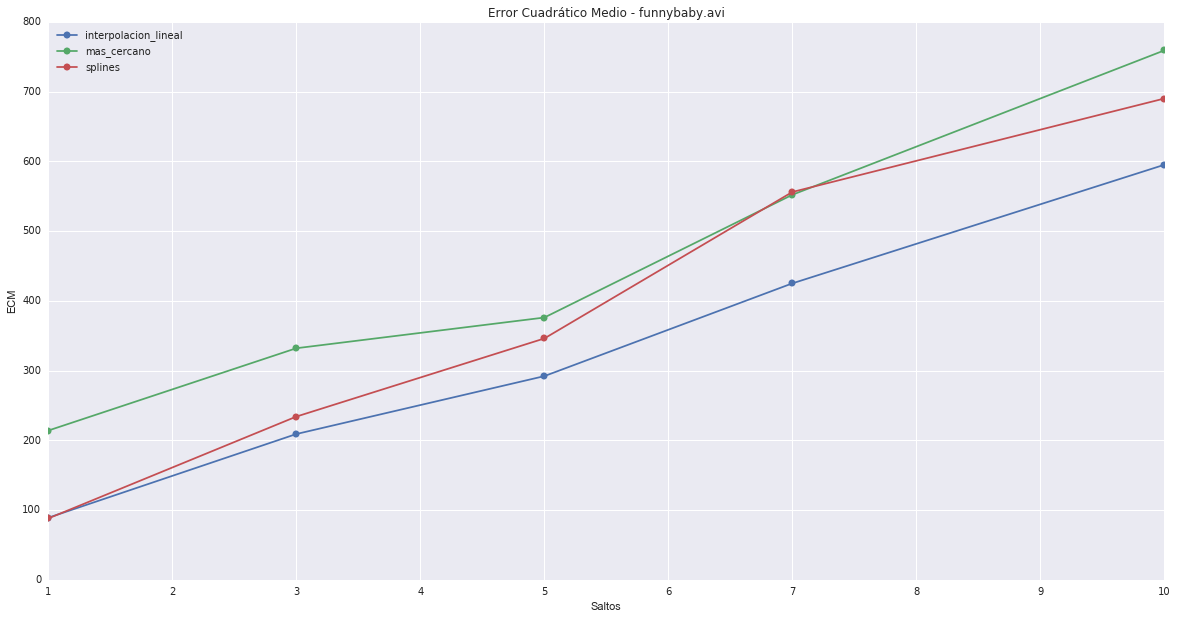
\includegraphics[width=.95\textwidth]{graficos/ecm_funnybaby.png}
\end{figure}

Como podemos ver, incre\'iblemente, en todos los videos el m\'etodo de \textbf{interpolaci\'on
lineal} es el que genera menores errores, inclusive menos que el de splines.

El an\'alisis por \textbf{PSNR} da un resultado similar al de \textbf{ECM}, ya
que los dos m\'etodos est\'an inversamente relacionados. Sin embargo, se nota
con m\'as claridad que cuando hay pocos saltos el resultado puede ser altamente
diferente.

\begin{figure}[H]
\centering
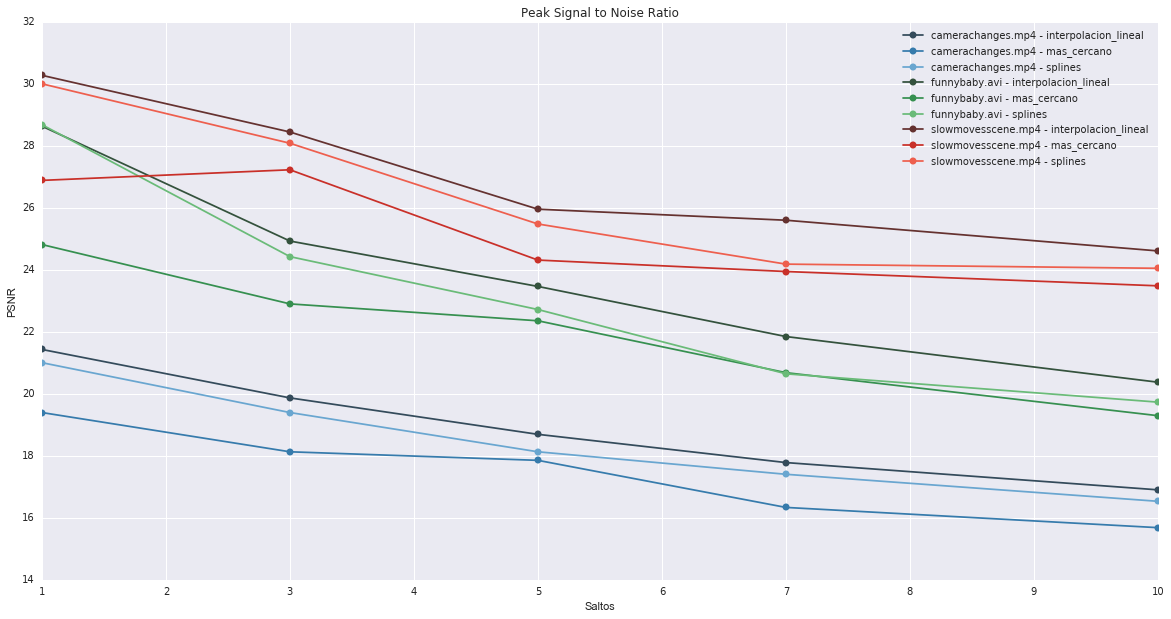
\includegraphics[width=.95\textwidth]{graficos/psnr.png}
\end{figure}
\vspace{-2em}
\begin{tiny}Este gr\'afico puede ser dificil de interpretar en blanco y negro\end{tiny}
\vspace{2em}

\subsubsection{An\'alisis de los m\'etodos frame por frame}

Como el calculo de \textbf{ECM}, que hasta ahora solo estamos promediando, se
hace por separado en cada frame, podemos hacer un an\'alisis por separado del
error medio en cada frame de algunos videos para poder encontrar cuanto cambiaba
este valor dependiendo de como se muevan, y si hay alg\'un m\'etodo que sea
preferible en alg\'un caso en particular.

Hicimos varias instancias de prueba similar a la del experimento anterior donde
habiendo un salto de \(2\) frames por cada frame del video original, ya que nos
parece una buena aproximaci\'on al caso real de alentizaci\'on de videos, y
calculamos el \textbf{ECM} entre cada uno de los frames generados y el frame
real.

\begin{figure}[H]
\centering
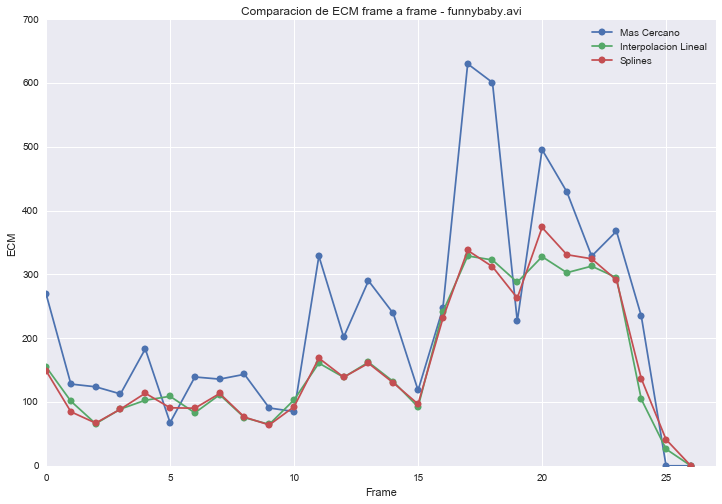
\includegraphics[width=.95\textwidth]{graficos/ecm_frame_funnybaby.png}
\end{figure}

Como \textit{funnybaby.avi} no tiene saltos ni ning\'un tipo de anormalidad en
todo el video, podemos ver que el \textbf{ECM} queda en el mismo orden de
magnitud por todo el an\'alisis. Sin embargo, podemos ver como este valor
aumenta considerablemente cuando el beb\'e del video hace una acci\'on que
cambia la mayor parte de los frames del video, como sacar la lengua o mover la
cabeza.

Al igual que en el an\'alisis del \textbf{ECM} promedio en el punto anterior,
con esta cantidad de saltos el valor de procesar el video con interpolaci\'on
lineal es similar a la de procesarlo con splines. Sin embargo, en este gr\'afico
tambi\'en se puede ver que aunque la diferencia entre el m\'etodo del m\'as
cercano con estos dos es similar cuando no hay muchos cambios, el error se
dispara cuando hay grandes cambios en la c\'amara.

Algo m\'as contundente pasa en el an\'alisis de otro video,
\textit{slowmovesscene.mp4}:

\begin{figure}[H]
\centering
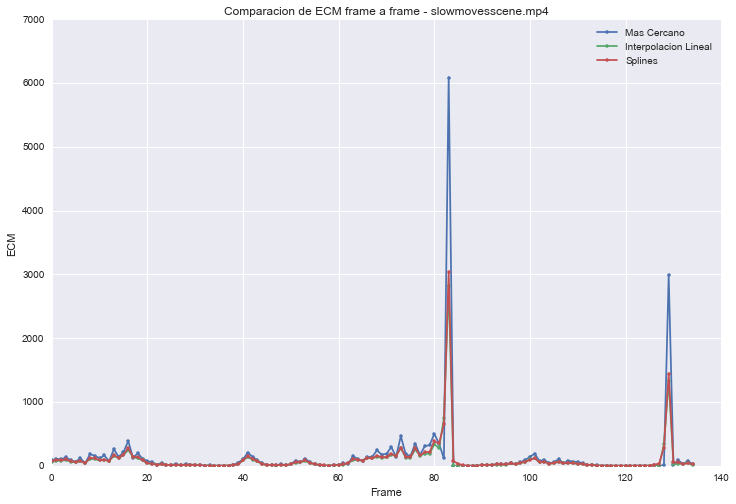
\includegraphics[width=.95\textwidth]{graficos/ecm_frame_slowmovescene.png}
\end{figure}

Este video tiene dos cambios de c\'amara importantes, y podemos ver que el
promedio del \textbf{ECM} se ve realmente afectado por los dos picos producidos
por estos cambios.

Como la distribuci\'on de los errores puede ser completamente diferente dentro y
fiera del pico, analizamos los dos casos por separado.

\begin{figure}[H]
\centering
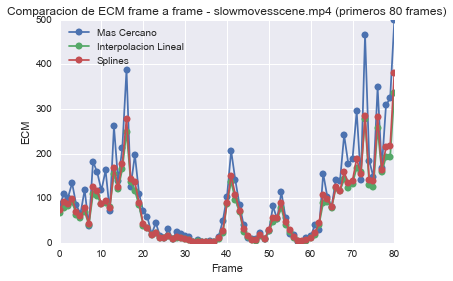
\includegraphics[width=.49\textwidth]{graficos/ecm_frame_slowmovescene_0_80.png}
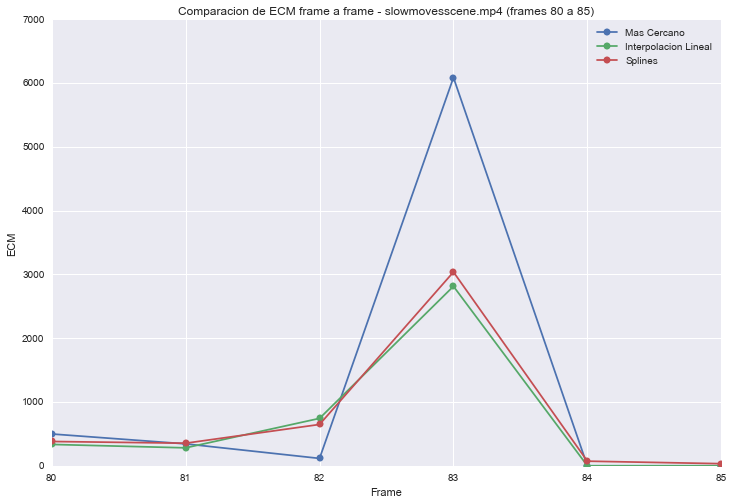
\includegraphics[width=.49\textwidth]{graficos/ecm_frame_slowmovescene_80_85.png}
\end{figure}

Podemos ver que en el gr\'afico que no incluye los picos tiene una
distribuci\'on similar a la de \textit{funnybaby.avi}, donde el m\'etodo de los
splines y el de interpolaci\'on lineal tienen resultados similares y el de
vecinos m\'as cercanos es considerablemente peor.

Sin embargo, haciendo zoom al pico m\'as grande, que pasa cuando la c\'amara
apunta al cielo, podemos varios patrones interesantes. Por ejemplo, el m\'etodo del
vecino m\'as cercano es el mejor por un solo frame cuando el video pasa por dos
frames seguidos en la misma imagen, ya que interpolaci\'on lineal y splines
intentan ser inteligentes y buscar un frame intermedio, mientras que el del
vecino m\'as cercano simplemente lo copia. Tambi\'en se puede ver que cuando se
hace el cambio de c\'amara, donde ninguno de los algoritmos puede predecir bien
cual va a ser el frame siguiente, el m\'etodo del vecino m\'as cercano es
considerablemente peor que los otros dos, y el de interpolaci\'on lineal es un
poco mejor al de splines.

\subsection{An\'alisis de la velocidad de los algoritmos}

\subsubsection{Comparaci\'on entre m\'etodos}

Todos los m\'etodos que usamos en la c\'amara lenta se aplican individualmente a
cada pixel, por lo tanto la complejidad temporal de los m\'etodos debe ser de la
forma $ \mathbb{O}(h \cdot w \cdot f^{(m)}(c_1)) $, con $h$ y $w$ alto y ancho del
video, respectivamente, $c_1$ la cantidad de frames del video final, y $f^{(m)}$
alguna funci\'on que depende del m\'etodo.

Como adem\'as ninguno de los tiempos de corrida de los m\'etodos cambia
dependiendo del valor de los pixeles \footnote{descontando el tiempo del
condicional cuando se pasa del rango de pixeles, que deber\'ia ser negligible},
una buena manera de medir la eficiencia de los m\'etodos es aplicandolos al
mismo video con diferente salto $s$ (ya que, para un $c_0$ fijo, tiene una
correlaci\'on lineal con $c_1$). Para este caso decidimos usar
\textit{baby.avi}.

Por cada m\'etodo, medimos la eficiencia de ese m\'etodo tomando el tiempo que
tarda en aplicar la c\'amara lenta a \textit{baby.avi} con diferentes 

\begin{figure}[H]
\centering
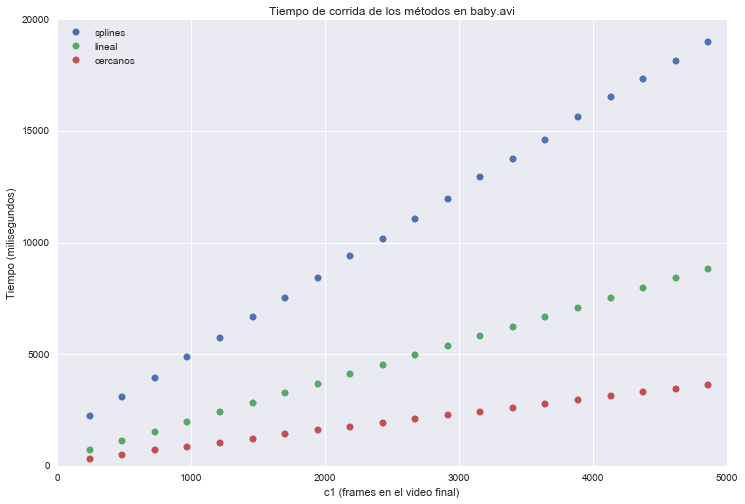
\includegraphics[width=.95\textwidth]{graficos/tiempo_baby.png}
\end{figure}

El gr\'afico da resultados previsibles: el tiempo de corrida del m\'etodo de los
splines es mayor que el de la interpolaci\'on lineal, que es mayor al de los
vecinos m\'as cercanos. Esto se debe a que, como explicado en el desarrollo,
el m\'etodo de los vecinos m\'as cercanos simplemente compia un valor de un
frame a otro y el de interpolaci\'on lineal hace una cuenta simple en punto
flotante, mientras que el de splines resuelve un sistema de $c_1$ ecuaciones.

Otra conclusi\'on que se puede sacar de este gr\'afico es que los tres m\'etodos
tiene complejidad temporal lineal. La raz\'on de esto es trivial en el caso de los
vecinos m\'as cercanos y el de la interpolaci\'on lineal, mientras que en el
caso de los splines nos aprovechamos que la matriz del sistema a resolver es
banda, lo que nos permite resolverlo en complejidad $\mathbb{O}(c_1)$ en vez de
la usual $\mathbb{O}(c_1^3)$.

\subsubsection{Reset en el m\'etodo de los splines}

Otro par\'ametro que puede tomar el \'ultimo m\'etodo, como est\'a explicado en
el desarrollo, es $r$, el ``reset'' del algoritmo. Esto indica que, en vez de
crear un sistema de ecuaciones para todos los puntos temporales en cada pixel,
va a crear sistemas de ecuaciones de tama\~no $r$ \footnote{posiblemente el
\'ultimo sea un poco m\'as grande}, y resolver cada sistema por separado.
Seg\'un nuestra hipotesis, esto deber\'ia resultar en un m\'etodo m\'as r\'apido
pero menos efectivo.

Para probarlo, dado que para probarlo eficientemente debemos hacerlo en videos
con un alto $c_1$, aprovechamos la propiedad de que el algoritmo funciona en
cada pixel por separado y creamos un video de tama\~no $1 \times 1$, con $c_0 =
100000$. De esta manera, podemos hacer las mismas pruebas m\'as r\'apido.

\begin{figure}[H]
\centering
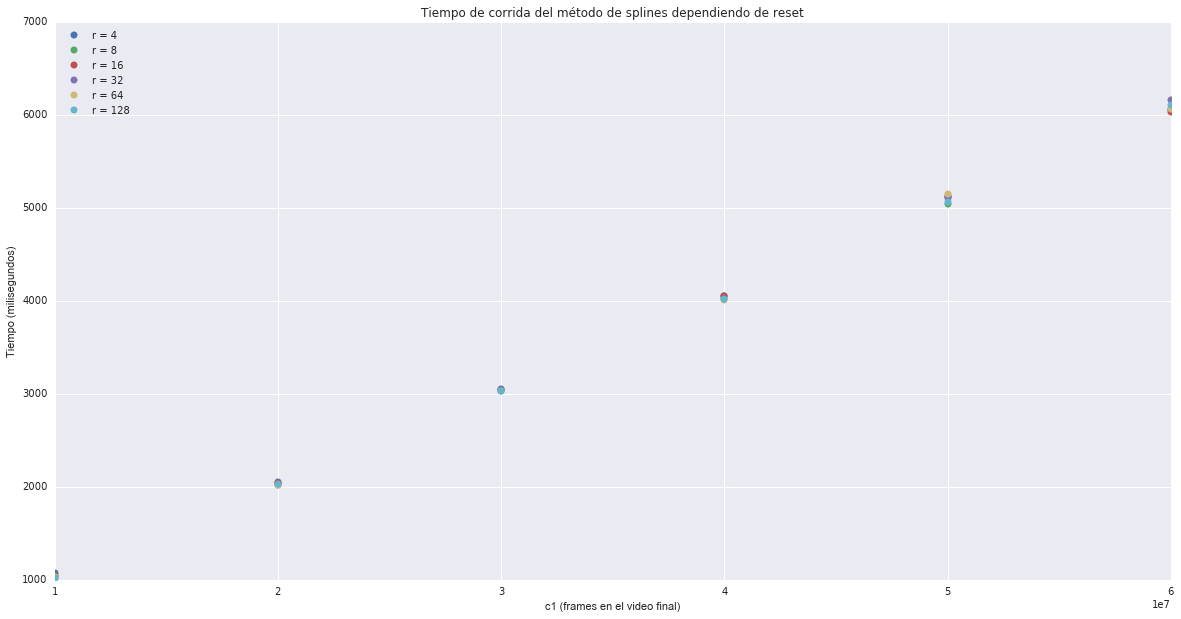
\includegraphics[width=.95\textwidth]{graficos/tiempo_reset.png}
\end{figure}

Por los resultados de los tiempos de la corrida podemos ver que nuestra
hip\'otesis es falsa. Al parecer, el algoritmo lineal para resolver el sistema
de ecuaciones con la matriz banda es lo suficientemente eficiente como para que
las ganancias de trabajar con matrices m\'as chicas sean negiglibles cuando se
les suma el costo de preparar y juntar las soluciones.

Por otro lado, analizando el \textbf{ECM} de estas instancias, podemos ver que
el resultado es peor que en una corrida del algoritmo de Splines sin usar reset,
y cuanto m\'as seguido se haga el reset mayor va a ser el error.

\begin{figure}[H]
\centering
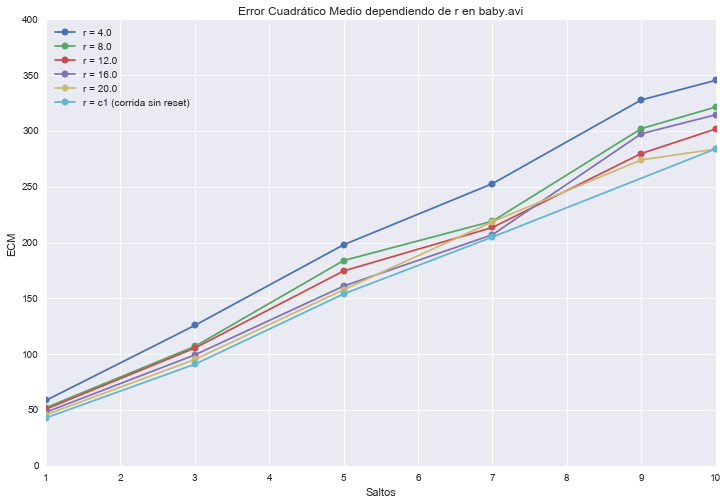
\includegraphics[width=.95\textwidth]{graficos/ecm_reset.png}
\end{figure}


\section{Conclusiones}

Luego de terminar la experimentaci\'on computacional y el an\'alisis de artifacts y otros efectos de video, deber\'iamos elegir el mejor m\'etodo entre los propuestos para alentar los videos.

Nos podemos guiar con los siguientes datos:

\begin{itemize}
	\item El m\'etodo de los vecinos m\'as cercanos, a pesar de ser el m\'as r\'apido de los m\'etodos, tiene un resultado con un error considerablemente mayor que los otros dos. Adem\'as, se pierde la fluidez y la ilusi\'on de movimiento continuo del video, as\'i que puede ser tranquilamente descartado entre los m\'etodos a usar.
	\item Cuando alenta el video un poco, hasta 3 o 4 veces el largo del video original, los m\'etodos de interpolaci\'on lineal e interpolaci\'on por splines tienen similar error cuadr\'atico medio, aunque es menor en el primer m\'etodo y en casi todos los frames. Cuando se alenta todav\'ia m\'as, la interpolaci\'on lineal pasa a ser considerablemente mejor que el caso de los splines.
	\item El m\'etodo de los splines es mucho m\'as lento que los otros dos m\'etodos, y separar los frames en grupos peque\~nos y calcular un spline por cada grupo no ayuda mucho a la velocidad, a pesar de hacer que el error sea todav\'ia mayor.
	\item El m\'etodo de interpolaci\'on por splines genera una cantidad considerale m\'as de artifacts que el de intepolaci\'on lineal, en especial cuando se consideran saltos de un valor alto.
	\item Aunque el error medio es mayor, cuando se analiza a ojo se puede notar que el m\'etodo de los splines es bastante m\'as flu\'ido que el de interpolaci\'on lineal. Esto se debe a que el cerebro humano analiza las imagenes de una manera bastante diferente que una computadora, y es una ventaja ya lo ideal es que el resultado sea visto por personas.
\end{itemize}

A pesar de que el \'ultimo punto aventaja ligeramente al m\'etodo de splines sobre el de interpolaci\'on lineal, nosotros llegamos a la conclusi\'on de que esta ventaja no supera a la mejoras sobre el tiempo de corrida y sobre error cuando el video se hace mucho m\'as lento que el original del segundo m\'etodo. Por lo tanto, en el caso general preferi\'iamos usar el m\'etodo de \textbf{interpolaci\'on lineal} para alentar un video.


\end{document}
